\begin{figure}[!tb]
\begin{center}
\begin{tikzpicture}[]
\fill (0,0) node[inner sep=1pt] (A) {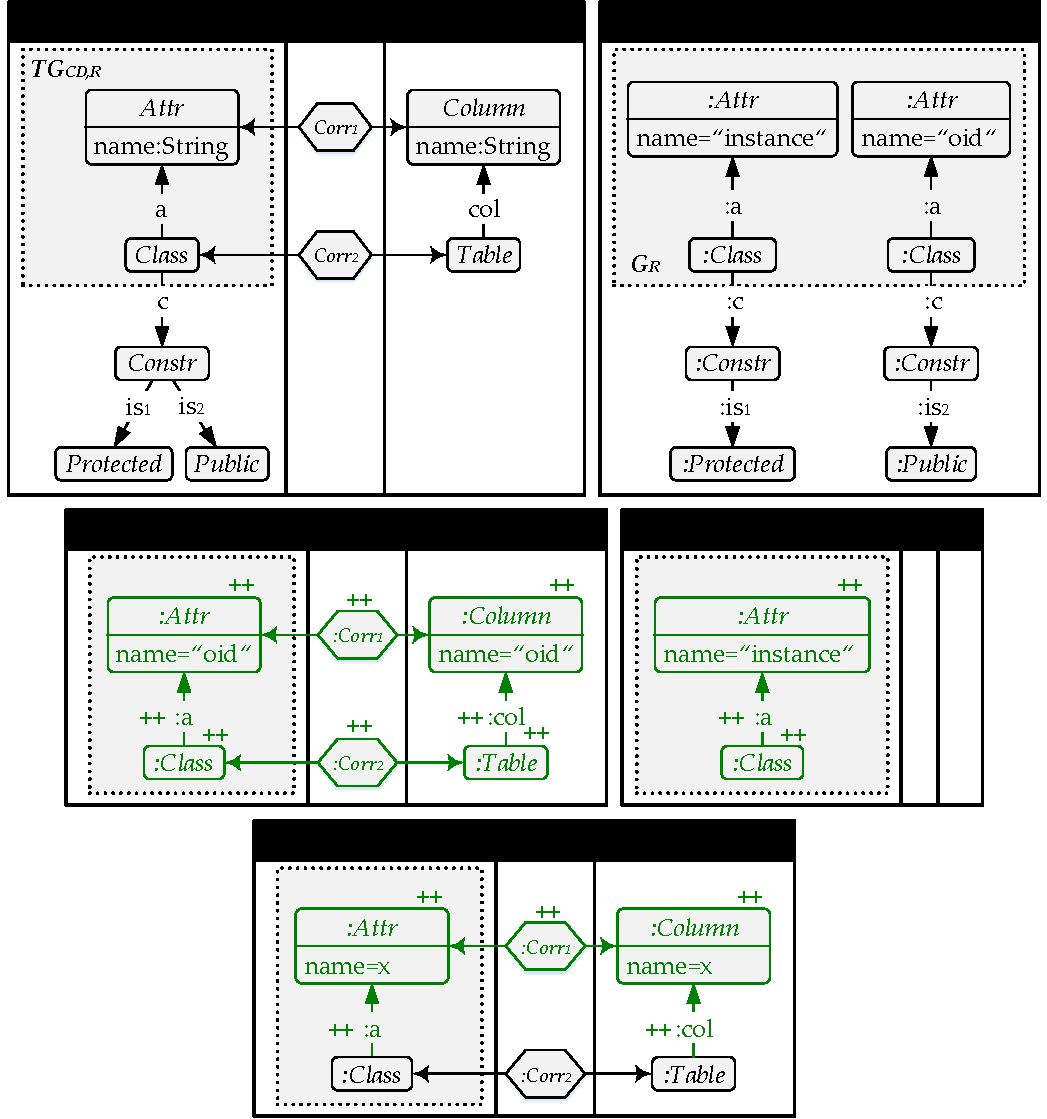
\includegraphics[width=\textwidth]{img/domain_res/res_tg.pdf}};
\fill (-2.5,7.55) node[inner sep=1pt] (B) {\textcolor{white}{$(\TG_\CD \gets \Corr \to \TG_\RDBM)$}};
\fill (1.4,7.55) node[inner sep=1pt] (C) {\textcolor{white}{$G$}};
\fill (-4.35,.4) node[inner sep=1pt] (D) {\textcolor{white}{InstantiableClass2Table}};
\fill (3,.4) node[inner sep=1pt] (E) {\textcolor{white}{Singleton2Empty}};
\fill (-2.55,-3.95) node[inner sep=1pt] (F) {\textcolor{white}{Attr2Column}};
\end{tikzpicture}
\end{center}
\caption{Triple Type Graph $(\TG_\CD \gets \Corr \to \TG_\RDBM)$ with Domain Restriction $\TG_{\CD,R}$ (top,left), Graph $G$ with Resitriction $G_R$ (top,right) and Triple Rules (bottom)}
\label{fig:sec-dc-general:res_tg}
\end{figure}

\begin{figure}[!tb]
\begin{center}
\begin{tikzpicture}[]
\fill (0,0) node[inner sep=1pt] (A) {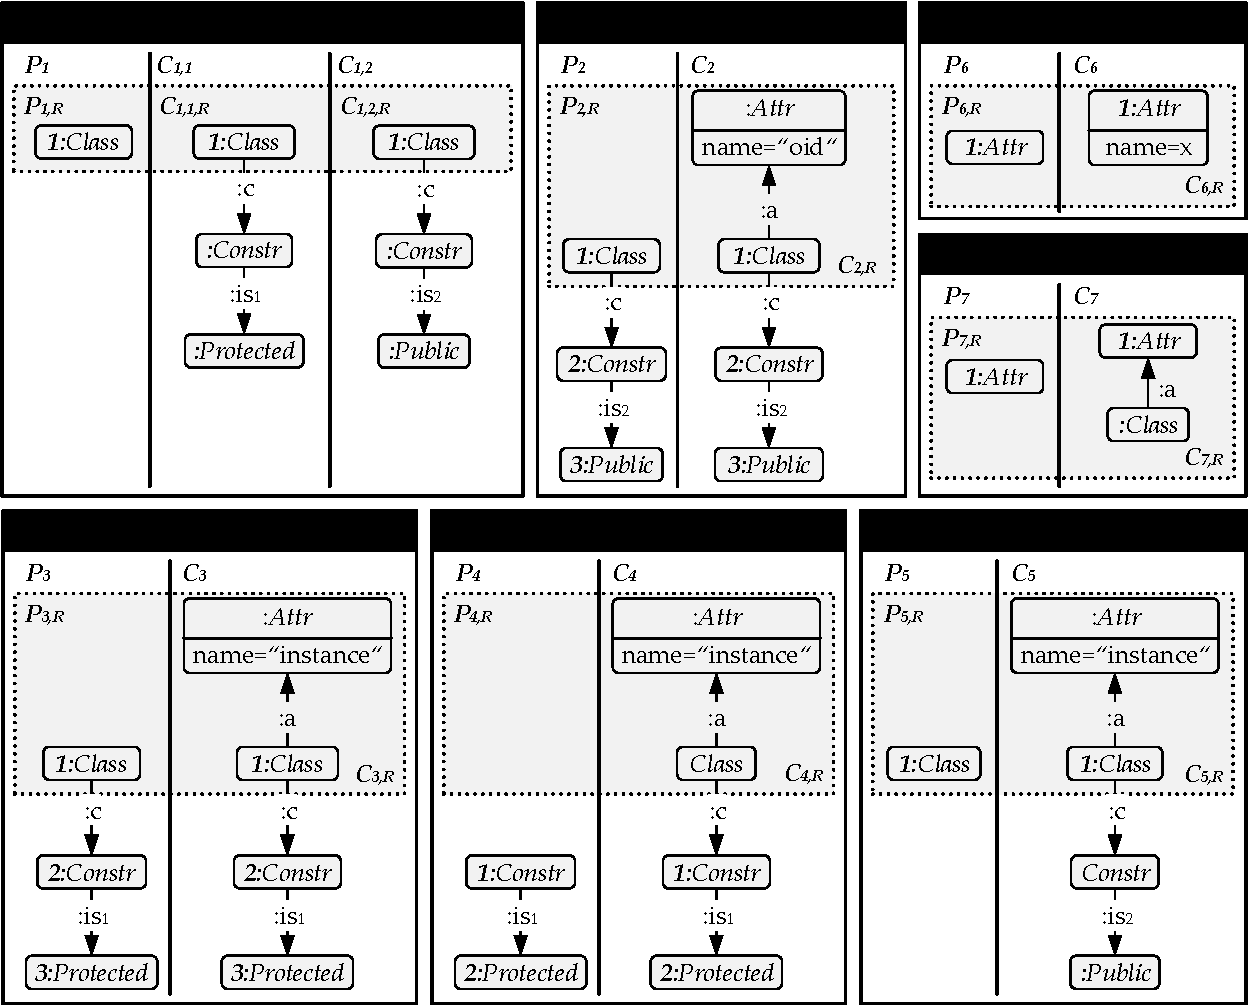
\includegraphics[width=\textwidth]{img/domain_res/res_c.pdf}};
\fill (-4.6,5.65) node[inner sep=1pt] (B) {\textcolor{white}{$c_1=\vee_{i=(1,2)}(\exists(P_1 \to C_{1,i},\true))$}};
\fill (.9,5.65) node[inner sep=1pt] (C) {\textcolor{white}{$c_2=\exists(P_2 \to C_2,\true)$}};
\fill (-5.45,-.35) node[inner sep=1pt] (D) {\textcolor{white}{$c_3=\exists(P_3 \to C_3,\true)$}};
\fill (-.4,-.35) node[inner sep=1pt] (E) {\textcolor{white}{$c_4=\exists(P_4 \to C_4,\true)$}};
\fill (4.8,-.35) node[inner sep=1pt] (F) {\textcolor{white}{$c_5=\neg\exists(P_5 \to C_5,\true)$}};
\fill (5.4,5.65) node[inner sep=1pt] (G) {\textcolor{white}{$c_6=\exists(P_6 \to C_6,\true)$}};
\fill (5.4,2.9) node[inner sep=1pt] (H) {\textcolor{white}{$c_7=\exists(P_7 \to C_7,\true)$}};
\end{tikzpicture}
\end{center}
\caption{Domain Graph Constraints with Restrictions}
\label{fig:sec-dc-general:res_c}
\end{figure}

According to \cref{sec-dom-compl}, we assume that the graphs (models) in the domain of discourse are defined by a domain type graph together with a set $C$ of domain graph constraints.
When verifying domain completeness w.r.t. a given graph grammar $\GG$, we may not be interested in a complete coverage of language $\Lang(C)$ by language $\Lang(\GG)$ but only in the coverage of certain elements of each graph in $\Lang(C)$ by $\Lang(\GG)$ which we call domain completeness under restrictions.
In \cref{fig:sec-dc-general:res_tg} we adress the translation of UML class diagrams (CDs) into relational database models (RDBMs) based on a triple graph grammar (TGG) (cf. \cref{sec-gen-intro-trafos}).
Therefore, the translation (TGG) only covers those elements $\TG_{\CD,R}$ in class diagrams that are related to RDBMs, i.e., classes and their attributes, while neglecting other details concerning class constructors and their visibilities.
However, the graph constraints restricting the structures of class diagrams may not only cover RDBM related elements but also other irrelevant elements for the translation.
This is problematic when verifying domain completeness under restrictions based on the techniques for verifying domain completeness in \cref{sec-dc-verification}, since, the extension of graphs via the constraints may lead to graphs with irrelevant elements that cannot be covered by the TGG causing the verification of $C$-extension completeness in \cref{def:C-extensionCompleteness} to fail.
In \cref{thm:sec-dc-general-res:dom_compl_res}, we give sufficient conditions under which the constraints can be restricted to relevant elements such that domain completeness under restrictions w.r.t. the original constraints can be verified based on the techniques for verifying domain completeness w.r.t. the restricted constraints in the sense of \cref{sec-dc-verification}.

\paragraph*{General Assumption:}
Initial and general satisfaction of constraints are defined over an initial object (cf. \cref{def:constr_sat}).
Therefore, we assume that the results of this Section are applied in the context of $\M$-adhesive categories with initial object.
Moreover, for the extension of constraints in \cref{thm:sec-dc-general-res:ext_constr}, we assume $\M$-adhesive categories with effective pushouts.

\paragraph*{}
For example, the triple type graph $(\TG_\CD \gets \Corr \to \TG_\RDBM)$ in \cref{fig:sec-dc-general:res_tg} (top,left) defines the model elements of class diagrams and database models.
Class diagrams (type graph $\TG_\CD$) may contain several \code{Class}es where each class may have an arbitrary number of \code{Attr}ibutes, each with a specific \code{name} of type \code{String}.
Furthermore, each class may have a \code{Constr}uctor with visibility \code{Protected} or \code{Public}.
Classes with protected constructors are singleton classes, i.e., there exists exactly one instance of each class.
In contrast, classes with public constructors are instantiable classes, i.e., there may exist an arbitrary number of instances of each class.
On the other hand, RDBMs (type graph $\TG_\RDBM$) may contain several \code{Table}s, each with an arbitrary number of \code{Column}s with a specific \code{name} of type \code{String}.
Moreover, classes (attributes) in CDs correspond to tables (columns) in RDBMs via $\Corr_2$ ($\Corr_1$) (cf. type graph $\Corr$).

Furthermore, the constraints in \cref{fig:sec-dc-general:res_c} state that
\begin{enumerate*}
\item each \code{Class} has a \code{Constr}uctor of visibility \code{Protected} or \code{Public} ($c_1=\vee_{i=(1,2)}(\exists(P_1 \to C_{1,i},\true))$),
\item each instantiable class has an \code{Attr}ibute ``\code{oid}'' (object id) which contains the unique id for each instantiated object of the class ($c_2=\exists(P_2 \to C_2,\true)$),
\item each singleton class has an attribute ``\code{instance}'' which contains the singleton instance object of the class ($c_3=\exists(P_3 \to C_3,\true)$),
\item each protected constructor is the constructor of some class with attribute ``instance'' ($c_4=\exists(P_4 \to C_4,\true)$ - Analogously, for public constructors a similar constraint is defined with attribute ``oid''),
\item each class is either singleton or instantiable, i.e., for each class there does not exist a public constructor and an attribute ``instance'' at the same time ($c_5=\neg\exists(P_5 \to C_5,\true)$ - Analogously, a similar constraint is defined for the combination of protected constructor and attribute ``oid''),
\item each attribute has a \code{name} ($c_6=\exists(P_6 \to C_6,\true)$), and
\item each attribute is assigned to a class ($c_7=\exists(P_7 \to C_7,\true)$).
\end{enumerate*}
Moreover, a constraint may be defined that prohibits classes to have protected and public constructors at the same time.

The triple rule \code{InstantiableClass2Table} in \cref{fig:sec-dc-general:res_tg} (bottom) defines the translation from CDs into RDBMs by mapping instantiable \code{Class}es with \code{Attr}ibute \code{oid} in CDs to corresponding \code{Table}s with \code{Column} \code{oid} in RDBMs.
Triple rule \code{Singleton2Empty} maps singleton \code{Classes} with \code{Attr}ibute \code{instance} in CDs to nothing in RDBMs, i.e., only instantiable classes are translated to corresponding tables whereas singleton classes are omitted.
Finally, triple rule \code{Attr2Column} translates general \code{Attr}ibutes with \code{name} ``\code{x}'' of \code{Class}es in CDs into \code{Columns} with the same name ``\code{x}" of corresponding \code{Table}s in RDBMs.

Therefore, the translation is restricted to (only covers) classes and attributes in CDs while neglecting constructors and their visibilities.
According to \cite{DBLP:journals/corr/abs-1209-1436}, the restriction is formalised by an $\M$-type morphism $t\colon \TG_{\CD,R} \to \TG_\CD \in \M$ from the restricted type graph $\TG_{\CD,R}$ which only contains classes and their attributes to the complete domain type graph $\TG_\CD$ of class diagrams (cf. \cref{fig:sec-dc-general:res_tg} (top,left)).
Therefore, each graph and graph constraint can be restricted along the type morphism while both may also contain elements outside the restriction, in general.
For example, graph $G_R$ in \cref{fig:sec-dc-general:res_tg} (top,right) is the restriction of graph $G$ along type morphism $t$ and constraints $c_i[P_i \mapsto P_{i,R},C_i \mapsto C_{i,R}]$ in \cref{fig:sec-dc-general:res_c} where premise (conclusion) $P_i$ ($C_i$) is substituted by $P_{i,R}$ ($C_{i,R}$) in each constraint are the restrictions of constraints $(c_i)_{i=(1..6)}$ along $t$.
The domain completeness problem under restrictions w.r.t. a given set of domain graph constraints $C$ and a graph grammar $\GG$ is as follows: Given a restriction of the domain type graph, does it hold for each graph $G$ in $\Lang(C)$ that the restriction of $G$ which comprises relevant elements only (i.e., elements that are typed over the restricted type graph) is covered by (contained in) grammar $\GG$ (language $\Lang(\GG)$)?

In the following, we first recall the definitions for rectrictions of graphs and positive (nested) graph constraints along type morphisms from \cite{DBLP:journals/corr/abs-1209-1436} and then we define the domain completeness problem under restrictions in accordance with the general domain completeness problem from \cref{def:sec-dc-general:dcp}.

%\vspace{2ex}
\parpic[r][r]{
\SelectTips{cm}{}
$
\xymatrix@C-4ex@R-4ex{
\TG & & G \ar[ll]_{t_G} & & G' \ar[ll]_{a} \\
& & & & \\
& (1) & & (2) & \\
& & & & \\
\TG_R \ar[uuuu]^{t} & & G_R \ar[ll]_{t_{G_R}} \ar[uuuu]^{t'} & & G'_R \ar[ll]_{a_R} \ar[uuuu]^{t''}
}
$
}
\vspace{-2ex}
\begin{definition}[Restriction along Type Morphism (Def. 3.1 \cite{DBLP:journals/corr/abs-1209-1436})]
\label{def:sec-dc-general-res:res_alomg_mor}
Given an object $(G,t_G)$ typed over $\TG$ via $t_G\colon G \to \TG$ and type morphism $t\colon \TG_R \to \TG \in \M$, then \emph{$\TG_R$ is called a restriction of $\TG$}\index{type graph!restriction} and \emph{$(G_R,t_{G_R})$ is a restriction of $(G,t_G)$ along $t$}\index{graph!restriction} with induced morphism $t'\colon G_R \to G$, written $G_R=\Restr_t(G)$, if $(1)$ is a pullback.
Given morphism $a\colon G' \to G$, then \emph{$a_R\colon G'_R \to G_R$ is a restriction of $a$ along $t$}\index{morphism!restriction}, written $a_R=\Restr_t(a)$, if additionally $(2)$ is a pullback.
\envEndMarker
\end{definition}

\begin{remark}[Restriction of Objects]
\label{rem:sec-dc-general-res:res_obj}
Note that by pullback composition with $(1)+(2)$ being a pullback, $(G'_R,t_{G_R} \circ a_R)$ is also a restriction of $(G',t_G \circ a)$ along $t$ with induced morphism $t''\colon G'_R \to G'$, written $G'_R=\Restr_t(G')$.
\envEndMarker
\end{remark}

\begin{definition}[Restriction of Nested Conditions (Def. 3.2 \cite{DBLP:journals/corr/abs-1209-1436})]
\label{def:sec-dc-general-res:res_cond}
Given a nested condition $\ac_P$ typed over $\TG$ and restriction $\TG_R$ of $\TG$ with type morphism $t\colon \TG_R \to \TG \in \M$.
Then, \emph{the restriction $\Restr_t(\ac_P)$ of $\ac_P$ along $t$}\index{graph condition!restriction} is defined as follows:
\begin{enumerate}
  \item $\Restr_t(\ac_P):=\true$ for $\ac_P=\true$,
  \item $\Restr_t(\ac_P):=\exists(\Restr_t(a), \Restr_t(\ac_C))$ for $\ac_P=\exists(a\colon P \to C,\ac_C)$,
  \item $\Restr_t(\ac_P):=\neg\Restr_t(\ac'_P)$ for $\ac_P=\neg\ac'_P$, and
  \item $\Restr_t(\ac_P):=(\vee_{i \in I})\wedge_{i \in I}(\Restr_t(\ac_{P,i}))$ for $\ac_P=(\vee_{i \in I})\wedge_{i \in I}(\ac_{P,i})$.
  \envEndMarker
\end{enumerate}
\end{definition}

\begin{definition}[Domain Completeness (Problem) under Restrictions]
\label{def:sec-dc-general-res:dc_prob}
Given the language $\Lang_I(C_I) \cap \Lang(C_G)$ over domain graph constraints $C=C_I \cup C_G$ and domain type graph $\TG$ with conditions $C_I$ ($C_G$) that are designated for initial (general) satisfaction.
Furthermore, let $t\colon \TG_R \to \TG \in \M$ be a type morphism such that $\TG_R$ is a restriction of $\TG$ and let $\Lang(\GG)$ be the language over graph grammer $\GG$ and restricted type graph $\TG_R$.
\emph{Domain completeness under restrictions}\index{domain completeness!under restrictions} holds if for all $G \in \Lang_I(C_I) \cap \Lang(C_G)$ it is true that $\Restr_t(G) \in \Lang(\GG)$.
Thus, the \emph{domain completeness problem under restrictions}\index{domain completeness!problem!under restrictions} is defined as follows: Does it hold that for all $G \in \Lang_I(C_I) \cap \Lang(C_G)$ it is true that $\Restr_t(G) \in \Lang(\GG)$?
\envEndMarker
\end{definition}

As already discussed at the beginning of this Section, in order to apply the results from \cref{sec-dc-verification} to the restricted domain type graph for verifying domain completeness under restrictions, the domain constraints need to be restricted at first.
However, the restriction of constraints may lead to constraints with a shifted meaning.
For example, when assuming general (initial) satisfaction for constraints, the restriction of constraints $c_2,c_3,c_4$ and $c_5$ in \cref{fig:sec-dc-general:res_c} lead to constraints with a meaning that was not prevailing before the restriction:
\begin{enumerate*}
\item The restriction of $c_2$ claims that each (there exists a) \code{Class} (that) has an \code{Attr}ibute \code{oid},
\item the restriction of $c_3$ claims that each (there exists a) \code{Class} (that) additionally has an \code{Attr}ibute \code{instance},
\item the restriction of $c_4$ claims that there exists a \code{Class} with \code{Attr}ibute \code{instance}, and
\item the restriction of $c_5$ claims that each (there exists a) \code{Class} (which) does not have an \code{Attr}ibute \code{instance}.
\end{enumerate*}
For general satisfaction, the restrictions of $c_2$ and $c_3$ lead to a contradiction in view of the unrestricted constraints, since, each class should be either singleton or instantiable by constraints $c_1$ and $c_5$.
Furthermore, the restriction of $c_4$ ($c_5$) prohibits class diagrams that only contain instantiable classes (or that contain singleton classes).
Similarly for initial satisfaction, the restrictions prohibit class diagrams that only contain instantiable or singleton classes.
Analogously, we obtain inconsistent results for the restrictions of negations $\neg c_2,\neg c_3$ and $\neg c_4$.
Thus, negations and constraints $\ac_P$ with elements in the premise graph $P$ that are outside the restriction may lead to inconsistent results when being restricted.
This is due to the fact that the context of elements in the premise (or conclusion) that is outside the restriction is lost after the restriction such that the restricted premise (or conclusion) may match to a wider range of graph patterns.

In the following, we show for the (general) initial satisfaction of positive graph constraints (which only contain restricted elements in their premises) that they can be restricted such that the restriction leads to a consistent result in the sense that each graph which satisfies the original constraint does also satisfy the restricted one as stated in \cref{lem:sec-dc-general-res:comp_res_sat_II}.
This extends the results in \cite{DBLP:journals/corr/abs-1209-1436} from initial to general satisfaction which is the usual interpretation of graph constraints, in particular in view of domain completeness (cf. \cref{sec-dc-general-lim}).
In \cref{lem:sec-dc-general-res:res_ob_sat}, we first prove that a graph $G$ initially (generally) satisfies a restricted condition $\Restr_t(\ac_P)$ if and only if its restriction $\Restr_t(G)$ initially (generally) satisfies $\Restr_t(\ac_P)$ which is used in the proof of \cref{lem:sec-dc-general-res:comp_res_sat_II}.

\begin{lemma}[Restriction of Objects and Satisfaction]
\label{lem:sec-dc-general-res:res_ob_sat}
Let $t\colon \TG_R \to \TG \in \M$ be a type morphism and $\TG_R$ be the restriction of type graph $\TG$.
Let $\ac_P$ be a nested condition typed over $\TG$, $\Restr_t(\ac_P)$ be its restriction along $t$, $(G,t_G\colon G \to \TG)$ be an object typed over $\TG$ via $t_G$ and $\Restr_t(G)$ be its restriction along $t$.
Then, $G \stackrel{I}{\models} \Restr_t(\ac_P)$ if and only if $\Restr_t(G) \stackrel{I}{\models} \Restr_t(\ac_P)$.
Furthermore, $G \models \Restr_t(\ac_P)$ if and only if $\Restr_t(G) \models \Restr_t(\ac_P)$.
\envEndMarker
\end{lemma}

\begin{proof}
The proof is presented in \cref{sec-proofs:lem:sec-dc-general-res:res_ob_sat}.
\end{proof}

In \cref{lem:sec-dc-general-res:comp_res_sat_I}, we show that if a graph $G$ generally satisfies a positive constraint $\ac_P$ where premise $P$ only contains elements within the restriction, then restricted graph $\Restr_t(G)$ also generally satisfies the restricted constraint $\Restr_t(\ac_P)$ which is used in the proof of \cref{lem:sec-dc-general-res:comp_res_sat_II}.
This extends the result for initial satisfaction from Cor. 5.2 in \cite{DBLP:journals/corr/abs-1209-1436} to general satisfaction.
In contrast to the result for initial satisfaction, \cref{lem:sec-dc-general-res:comp_res_sat_I} does not hold for positive constraints with elements in the premise that are outside the restriction, in general, as shown by the following counter-example.
Consider constraint $c_3$ in \cref{fig:sec-dc-general:res_c}.
Given a class diagram with instantiable classes only that generally satisfies $c_3$, then the restriction of the class diagram according to $\TG_{\CD,R}$ in \cref{fig:sec-dc-general:res_tg} may not generally satisfy the restricted constraint $\Restr_t(c_3)$, since, there may be classes without an attribute of name \code{instance}.
Furthermore, similarly to the result for initial satisfaction, \cref{lem:sec-dc-general-res:comp_res_sat_I} does not hold for non-positive constraints even if the premise only contains elements within the restriction, in general (cf. constraint $c_5$ in \cref{fig:sec-dc-general:res_c}).
\cref{lem:sec-dc-general-res:comp_res_sat_I} holds for constraints $c_1,c_6$ and $c_7$ in \cref{fig:sec-dc-general:res_c}, since, these constraints are positive and only contain elements in their premises $P_1,P_6$ and $P_7$ that are within the restriction.
Before proving \cref{lem:sec-dc-general-res:comp_res_sat_I}, we prove \cref{lem:sec-dc-general-res:comp_res_sat_mor} which is used in the proof of \cref{lem:sec-dc-general-res:comp_res_sat_I}.

\begin{lemma}[Compatibility of Restriction and General Satisfaction I]
\label{lem:sec-dc-general-res:comp_res_sat_mor}
Let $t\colon \TG_R \to \TG \in \M$ be a type morphism and $\TG_R$ be the restriction of type graph $\TG$.
Let $\ac_P$ be a positive nested condition over premise $P$ and typed over $\TG$ and $\Restr_t(\ac_P)$ be its restriction over $\Restr_t(P)$ along $t$ with induced morphism $i\colon \Restr_t(P) \to P$.
Given an object $(G,t_G\colon G \to \TG)$ typed over $\TG$ via $t_G$ and its restriction $\Restr_t(G)$ along $t$ with induced morphism $t'\colon \Restr_t(G) \to G$.
Then, it holds that if there is $p\colon P \to G \in \M$ with $p \models \ac_P$, then there is a unique $p_R\colon \Restr_t(P) \to \Restr_t(G) \in \M$ such that $t' \circ p_R=p \circ i$.
Furthermore, it holds that $p_R \models \Restr_t(\ac_P)$.
\envEndMarker
\end{lemma}

\begin{proof}
Let $p \in \M$ with $p \models \ac_P$.
By construction of $\Restr_t(G)$, $(3)$ is a pullback (PB) with $t' \in \M$ (cf. \cref{def:sec-dc-general-res:res_alomg_mor}), since, $\M$-morphisms $t \in \M$ are closed under pullbacks.
By induction over the structure of nested conditions:
\textbf{Basis.}
Let $\ac_P=\true=\Restr_t(\ac_P)$.
By construction of $\Restr_t(P)$, $(1)+(2)$ is a pullback.
By $p$ being a morphism and $G,P$ both being typed over $\TG$ via $t_G$ and $t_C \circ a$ it follows that $t_G \circ p=t_C \circ a$ $^{(*^1)}$.
Thus, $t_G \circ p \circ i$ $\stackrel{(*^1)}{=}$ $t_C \circ a \circ i$ $\stackrel{PB (1)+(2)}{=}$ $t \circ t_{C_R} \circ a_R$.
By the universal property of pullback $(3)$, there is a unique $p_R$ with $t' \circ p_R=p \circ i$ and $p_R \models \true=\Restr_t(\ac_P)$.
By $\M$-morphisms $t \in \M$ are closed under pullbacks $(1)+(2)$, $i \in \M$.
By $\M$-composition, $p \circ i \in \M$ and therefore, by $\M$-decomposition with $t' \in \M$, $p_R \in \M$.
\begin{center}
\begin{tikzpicture}[]
\fill (0,0) node[inner sep=1pt] (TG) {$\TG$};
\fill (0,0) node[right of=TG,xshift=2cm,inner sep=1pt] (C) {$C$};
\fill (0,0) node[right of=C,xshift=2cm,inner sep=1pt] (P) {$P$};
\fill (0,0) node[below of=TG,yshift=-1cm,inner sep=1pt] (TGR) {$\TG_R$};
\fill (0,0) node[right of=TGR,xshift=2cm,inner sep=1pt] (CR) {$\Restr_t(C)$};
\fill (0,0) node[right of=CR,xshift=2cm,inner sep=1pt] (PR) {$\Restr_t(P)$};
\fill (0,0) node[left of=TG,xshift=-2cm,inner sep=1pt] (G) {$G$};
\fill (0,0) node[left of=TGR,xshift=-2cm,inner sep=1pt] (GR) {$\Restr_t(G)$};
%
\fill (0,0) node[right of=G,xshift=.5cm,yshift=-1cm,inner sep=1pt] (3) {$(3)$};
\fill (0,0) node[right of=TG,xshift=.5cm,yshift=-1cm,inner sep=1pt] (1) {$(1)$};
\fill (0,0) node[right of=C,xshift=.5cm,yshift=-1cm,inner sep=1pt] (2) {$(2)$};
%
\fill (0,0) node[above of=C,yshift=-.4cm,isosceles triangle, fill=gray!25,draw,shape border rotate=270,minimum width=0.4cm, inner sep=1pt] (t) {};
\fill (0,0) node[above of=C,yshift=-.1cm,inner sep=1pt] {$\ac_C$};
\fill (0,0) node[below of=CR,yshift=.4cm,isosceles triangle, fill=gray!25,draw,shape border rotate=90,minimum width=0.4cm, inner sep=1pt] (t) {};
\fill (0,0) node[below of=CR,yshift=.1cm,inner sep=1pt] {$\Restr_t(\ac_C)$};
%
{
\pgfsetarrowsend{latex}
\draw (C) -> node[fill=white,inner sep=1pt]{$\scriptstyle{t_C}$} (TG);
\draw (CR) -> node[fill=white,inner sep=1pt]{$\scriptstyle{t_{C_R}}$} (TGR);
\draw (P) -> node[fill=white,inner sep=1pt]{$\scriptstyle{a}$} (C);
\draw (PR) -> node[fill=white,inner sep=1pt]{$\scriptstyle{a_R}$} (CR);
\draw (G) -> node[fill=white,inner sep=1pt]{$\scriptstyle{t_G}$} (TG);
\draw (GR) -> node[fill=white,inner sep=1pt]{$\scriptstyle{t_{G_R}}$} (TGR);
\draw (GR) -> node[fill=white,inner sep=1pt]{$\scriptstyle{t'}$} (G);
\draw (CR) -> node[fill=white,inner sep=1pt]{$\scriptstyle{t''}$} (C);
\draw (TGR) -> node[fill=white,inner sep=1pt]{$\scriptstyle{t}$} (TG);
\draw (PR) edge[bend left=20] node[fill=white,inner sep=1pt]{$\scriptstyle{i}$} (P);
\draw (P) edge[bend left=20] node[fill=white,inner sep=1pt]{$\scriptstyle{i^{-1}}$} (PR);
\draw (C) edge[bend right=15] node[fill=white,inner sep=1pt]{$\scriptstyle{q}$} (G);
\draw (P) edge[bend right=35] node[fill=white,inner sep=1pt]{$\scriptstyle{p}$} (G);
\draw (CR) edge[dotted,bend left=15] node[fill=white,inner sep=1pt]{$\scriptstyle{q_R}$} (GR);
\draw (PR) edge[dotted,bend left=35] node[fill=white,inner sep=1pt]{$\scriptstyle{p_R}$} (GR);
\pgfsetarrows{right hook-latex}
%
\pgfsetarrows{*-latex}
%
}
\end{tikzpicture}
\end{center}
\textbf{Hypothesis.}
The assumption holds for positive conditions $\ac_C,\ac_{P,i},i \in I$ and their restrictions $\Restr_t(\ac_C),\Restr_t(\ac_{P,i})$.
\textbf{Step.}
Let $\ac_P=\exists(a\colon P \to C,\ac_C)$ and $\Restr_t(\ac_P)=\exists(a_R\colon \Restr_t(P) \to \Restr_t(C),\Restr_t(\ac_C))$ with pullbacks $(1)$ and $(2)$ by the construction of restrictions of conditions (cf. \cref{def:sec-dc-general-res:res_cond}).
Pullback composition implies that $(1)+(2)$ is a pullback.
Analogously to the induction basis, there is a unique $p_R \in \M$ with $t' \circ p_R=p \circ i$ $^{(*^3)}$.
By assumption $p \models \ac_P$, there is $q \in \M$ with $q \circ a=p$ and $q \models \ac_C$ $^{(*^4)}$.
By $q$ being a morphism and $G,C$ being typed over $\TG$ via $t_G,t_C$, $t_G \circ q=t_C$ $^{(*^2)}$.
Thus, $t_g \circ q \circ t''$ $\stackrel{(*^2)}{=}$ $t_C \circ t''$ $\stackrel{PB (1)}{=}$ $t \circ t_{C_R}$.
By the universal property of pullback $(3)$, there is a unique $q_R$ with $t' \circ q_R=q \circ t''$ $^{(*^5)}$.
Furthermore, $q_R \in \M$, since, $t'' \in \M$ by $\M$-morphisms $t \in \M$ are closed under pullbacks $(1)$, $q \circ t'' \in \M$ by $\M$-composition and $q_R \in \M$ by $\M$-decomposition with $t' \in \M$ and $(*^5)$.
Thus, $t' \circ q_R \circ a_R$ $\stackrel{(*^5)}{=}$ $q \circ t'' \circ a_R$ $\stackrel{PB (2)}{=}$ $q \circ a \circ i$ $\stackrel{(*^4)}{=}$ $p \circ i$ $\stackrel{(*^3)}{=}$ $t' \circ p_R$.
By $t' \in \M$ being a monomorphism, $q_R \circ a_R=p_R$.
Furthermore, by induction hypothesis, $q_R \models \Restr_t(\ac_C)$.
Therefore, $p_R \models \Restr_t(\ac_P)$.

For conditions $\ac_P=\wedge_{i \in I}(\ac_{P,i})$ we conclude as follows.
Assumption $p \models \ac_P$ implies that $p \models \ac_{P,i}$ for all $i \in I$.
Therefore, there is a unique $p_R \in \M$ with $t' \circ p_R=p \circ i$ and $p_R \models Restr_t(\ac_{P,i})$ for all $i \in I$ implying further that $p_R \models \wedge_{i \in I}(Restr_t(\ac_{P,i}))=\Restr_t(\ac_P)$.
Analogously, we prove the assumption for conditions $\ac_P=\vee_{i \in I}(\ac_{P,i})$.
\end{proof}

\begin{lemma}[Compatibility of Restriction and General Satisfaction II]
\label{lem:sec-dc-general-res:comp_res_sat_I}
Let $t\colon \TG_R \to \TG \in \M$ be a type morphism and $\TG_R$ be the restriction of type graph $\TG$.
Let $\ac_P$ be a positive nested condition over premise $P$ and typed over $\TG$ with $P \cong \Restr_t(P)$ and $\Restr_t(\ac_P)$ be its restriction over $\Restr_t(P)$ along $t$.
Given an object $(G,t_G\colon G \to \TG)$ typed over $\TG$ via $t_G$ and its restriction $\Restr_t(G)$ along $t$ with induced morphism $t'\colon \Restr_t(G) \to G$, then it holds that $G \models \ac_P \implies \Restr_t(G) \models \Restr_t(\ac_P)$.
\envEndMarker
\end{lemma}

\begin{proof}
Based on the figure in the proof of \cref{lem:sec-dc-general-res:comp_res_sat_mor}, by induction over the structure of nested conditions:
\textbf{Basis.}
For $\ac_P=\true=\Restr_t(\ac_P)$, for all $p_R\colon \Restr_t(P) \to \Restr_t(G)$ it holds that $p_R \models \Restr_t(\ac_P)$, i.e., $\Restr_t(G) \models \Restr_t(\ac_P)$.

We show for $\ac_P=\exists(a\colon P \to C,\ac_C)$ and its restriction $\Restr_t(\ac_P)=\exists(a_R\colon \Restr_t(P) \to \Restr_t(C),\Restr_t(\ac_C))$ that if $G \models \ac_P$, then for all $p_R\colon \Restr_t(P) \to \Restr_t(G) \in \M$ there is $q_R\colon \Restr_t(C) \to \Restr_t(G) \in \M$ with $q_R \circ a_R=p_R$ and $q_R \models \Restr_t(\ac_C)$.
This directly implies that $\Restr_t(G) \models \Restr_t(\ac_P)$.
Let $P \cong Restr_t(P)$ with (inverse) isomorphism $i\colon \Restr_t(P) \to P$ ($i^{-1}\colon P \to \Restr_t(P)$) and $i,i^{-1} \in \M$, since, class $\M$ contains all isomorphisms.
Let $p_R \in \M$.
There is $p=t' \circ p_R \circ i^{-1} \in \M$ by $\M$-composition and $t',t'' \in \M$, since, pullbacks (PBs) $(3)$ and $(1)$ preserves $\M$-morphisms $t \in \M$ $\stackrel{G \models \ac_P}{\Rightarrow}$ There is $q\colon C \to G \in \M$ with $q \models \ac_C$ and $q \circ a=p=t' \circ p_R \circ i^{-1}$ $^{(*^1)}$.
By $q$ being a morphism, $t_G \circ q=t_C$ $\Rightarrow$ $t_G \circ q \circ t''=t_C \circ t''$ $\stackrel{PB (1)}{=}$ $t \circ t_{C_R}$.
By the universal property of pullback $(3)$, there is a unique $q_R\colon \Restr_t(C) \to \Restr_t(G)$ with $t' \circ q_R=q \circ t''$ $^{(*^2)}$.
Furthermore, $q_R \in \M$ by first $\M$-composition with $t' \circ q_R=q \circ t'' \in \M$ and then, $\M$-decomposition with additionally $t' \in \M$.
Thus, $t' \circ p_R$ $\stackrel{i\text{ is isomorphism}}{=}$ $p \circ i$ $\stackrel{(*^1)}{=}$ $q \circ a \circ i$ $\stackrel{PB (2)}{=}$ $q \circ t'' \circ a_R$ $\stackrel{(*^2)}{=}$ $t' \circ q_R \circ a_R$ $\stackrel{t'\in\M\text{ is a monomorphism}}{\Rightarrow}$ $q_R \circ a_R=p_R$.
Furthermore, by \cref{lem:sec-dc-general-res:comp_res_sat_mor}, $q_R \models \Restr_t(\ac_C)$.
Thus, $p_R \models \Restr_t(\ac_P)$ and furthermore, $\Restr_t(G) \models \Restr_t(\ac_P)$.
\textbf{Hypothesis.}
The assumption holds for conditions $\ac_{P,i},i \in I$ and their restrictions $\Restr_t(\ac_{P,i})$.
\textbf{Step.}
Let condition $ac_P=\wedge_{i \in I}(\ac_{P,i})$.
Assumption $G \models \ac_P$ implies that $G \models \ac_{P,i}$ for all $i \in I$.
By induction hypothesis, $\Restr_t(G) \models \Restr_t(\ac_{P,i})$ for all $i \in I$.
Therefore, $\Restr_t(G) \models \wedge_{i \in I}(\Restr_t(\ac_{P,i}))=\Restr_t(\ac_P)$.
For conditions $ac_P=\vee_{i \in I}(\ac_{P,i})$ we conclude analogously.
\end{proof}

In \cref{lem:sec-dc-general-res:comp_res_sat_II}, we give  sufficient conditions under which constraints can be restricted such that each graph which initially (generally) satisfies the original constraint does also initially (generally) satisfy the restricted one.
Therefore, the domain constraints can be restricted such that all graphs that satisfy the original domain constraints do also satisfy the restricted domain constraints.
Thus, (a successful verification of) domain completeness under restrictions w.r.t. the restricted constraints implies domain completeness under restrictions w.r.t. the original constraints which can be verified based on the techniques from \cref{sec-dc-verification} for verifying ``standard" domain completeness w.r.t. the restricted constraints as stated in \cref{thm:sec-dc-general-res:dom_compl_res}.

\begin{proposition}[Compatibility of Restriction and Satisfaction]
\label{lem:sec-dc-general-res:comp_res_sat_II}
Let $t\colon \TG_R \to \TG \in \M$ be a type morphism and $\TG_R$ be the restriction of type graph $\TG$.
Let $\ac_P$ be a positive nested condition over premise $P$ and typed over $\TG$ and $\Restr_t(\ac_P)$ be its restriction along $t$.
Given an object $(G,t_G\colon G \to \TG)$ typed over $\TG$ via $t_G$, then it holds that $G \stackrel{I}{\models} \ac_P \implies G \stackrel{I}{\models} \Restr_t(\ac_P)$.
Furthermore, if $P \cong \Restr_t(P)$, then $G \models \ac_P \implies G \models \Restr_t(\ac_P)$.
For a set $C=C_I \cup C_G$ of positive nested conditions typed over $\TG$ with conditions $C_I$ ($C_G$) that are designated for initial (general) satisfaction and furthermore, with $P \cong \Restr_t(P)$ for all $\ac_P \in C_G$ it holds that $\Lang_I(C_I) \cap \Lang(C_G) \subseteq \Lang_I(\Restr_t(C_I)) \cap \Lang(\Restr_t(C_G))$ where $\Restr_t(C):=\{\Restr_t(c) \mid c \in C\}$.
\envEndMarker
\end{proposition}

\begin{proof}
We first show the result for initial satisfaction and for general satisfaction afterwards.
\begin{enumerate}
  \item[``$\stackrel{I}{\models}$''] Let $G \stackrel{I}{\models} \ac_P$, i.e., there exists $p\colon P \to G \in \M$ with $p \models \ac_P$.
  By Fact 3.4 in \cite{DBLP:journals/corr/abs-1209-1436}, there exists $p_R\colon \Restr_t(P) \to \Restr_t(G) \in \M$ with $p_R \models \Restr_t(\ac_P)$.
  By the uniquness of initial morphisms, for initial object $I$ and initial morphisms $i_1\colon I \to \Restr_t(P)$, $i_2\colon I \to \Restr_t(G)$ we obtain that $p_R \circ i_1=i_2$ and therefore, $\Restr_t(G) \stackrel{I}{\models} \Restr_t(\ac_P)$.
  By \cref{lem:sec-dc-general-res:res_ob_sat}, $G \stackrel{I}{\models} \Restr_t(\ac_P)$.
  \item[``$\models$''] $G \models \ac_P$ $\stackrel{\cref{lem:sec-dc-general-res:comp_res_sat_I}}{\Rightarrow}$ $\Restr_t(G) \models \Restr_t(\ac_P)$ $\stackrel{\cref{lem:sec-dc-general-res:res_ob_sat}}{\Rightarrow}$ $G \models \Restr_t(\ac_P)$.
\end{enumerate}
Finally, $G \in \Lang_I(C_I) \cap \Lang(C_G)$ implies that $G \stackrel{I}{\models} c_I$ and $G \models c_G$ for all $c_I \in C_I,c_G \in C_G$ implying further that $G \stackrel{I}{\models} \Restr_t(c_I)$ and $G \models \Restr_t(c_G)$ for all $c_I \in C_I,c_G \in C_G$.
Therefore, $G \in \Lang_I(\Restr_t(C_I)) \cap \Lang(\Restr_t(C_G))$, i.e., $\Lang_I(C_I) \cap \Lang(C_G) \subseteq \Lang_I(\Restr_t(C_I)) \cap \Lang(\Restr_t(C_G))$.
\end{proof}

Beside conditions with premises that only contain elements within the restrictions, we define conditions that are already purely restricted not only for the premise but also for all conclusions, called purely restricted conditions.
\cref{lem:sec-dc-general-res:comp_res_sat_III,prop:sec-dc-general-res:comp_res_sat_III} state that a purely restricted condition and its restriction are semantically equivalent.
While in \cref{lem:sec-dc-general-res:comp_res_sat_II} we restrict to positive conditions only, in \cref{prop:sec-dc-general-res:comp_res_sat_III} we restrict to possibly non-positive conditions with negations that are purely restricted and show that these conditions can be directly used for verifying domain completeness under restrictions as stated in \cref{thm:sec-dc-general-res:dom_compl_res}.
For example, conditions $c_6$ and $c_7$ in \cref{fig:sec-dc-general:res_c} is purely restricted while condition $c_1$ is not.
Although $c_1$ only contains elements in its premise that are within the restriction, it is not purely restricted, since, conclusions $C_{1,1}$ and $C_{1,2}$ also contain elements that are outside the restriction.

\begin{definition}[(Purely) Restricted Condition]
Let $t\colon \TG_R \to \TG \in \M$ be a type morphism and $\TG_R$ be the restriction of type graph $\TG$.
Let $\ac_P$ be a nested condition over premise $P$ and typed over $\TG$.
\emph{Condition $\ac_P$ is purely restricted along $t$}\index{graph condition!purely restricted}, if for all morphisms $a\colon P' \to C'$ in $\ac_P$ and their restrictions $\Restr_t(a)\colon \Restr_t(P') \to \Restr_t(C')$ it holds that the induced morphisms in \cref{def:sec-dc-general-res:res_alomg_mor} are isomorphisms, i.e., $P' \cong \Restr_t(P')$ and $C' \cong \Restr_t(C')$.
\emph{Condition $\ac_P$ is restricted along $t$}\index{graph condition!restricted}, if $P \cong \Restr_t(P)$.
\envEndMarker
\end{definition}

\begin{lemma}[Compatibility of Pure Restrictions and General Satisfaction]
\label{lem:sec-dc-general-res:comp_res_sat_III}
Let $t\colon \TG_R \to \TG \in \M$ be a type morphism and $\TG_R$ be the restriction of type graph $\TG$.
Let $\ac_P$ be a purely restricted condition along $t$ over premise $P$ and typed over $\TG$ and $\Restr_t(\ac_P)$ be its restriction over $\Restr_t(P)$ along $t$ with induced morphism $i\colon \Restr_t(P) \to P$.
Given an object $(G,t_G\colon G \to \TG)$ typed over $\TG$ via $t_G$.
Then, it holds that:
\begin{enumerate}
  \item \label{item:sec-dc-general-res:comp_res_sat_III:1} If there is $p\colon P \to G \in \M$ with $p \models \ac_P$, then there is a unique morphism $p_R\colon \Restr_t(P) \to G \in \M$ such that $p_R=p \circ i$.
  Furthermore, $p_R \models \Restr_t(\ac_P)$.
  \item \label{item:sec-dc-general-res:comp_res_sat_III:2} If there is $p_R\colon \Restr_t(P) \to G \in \M$ with $p_R \models \Restr_t(\ac_P)$, then there is a unique morphism $p\colon P \to G \in \M$ such that $p_R=p \circ i$.
  Furthermore, $p \models \ac_P$.
\end{enumerate} 
\envEndMarker
\end{lemma}

\begin{proof}
By the construction of restrictions, $(1)$ and $(2)$ are pullbacks (cf. \cref{def:sec-dc-general-res:res_alomg_mor}).
Furthermore, by assumption $\ac_P$ is purely restricted, induced morphisms $t''$ and $i$ are isomorphisms with inverse isomorphisms $t''^{-1}$ and $i^{-1}$.
Moreover, $t'',i \in \M$, since, $\M$-morphisms $t \in \M$ are closed under pullbacks $(1),(2)$.
We first show the result for positive conditions and for negations afterwards.
\begin{enumerate}
  \item Let $p_R=p \circ i$.
  The uniqueness of $p_R$ directly follows by definition - Assume $p'_R$ such that $p'_R=p \circ i$, then $p'_R=p \circ i=p_R$.
  Furthermore, $p_R \in \M$ by $\M$-composition of $p,i \in \M$.
  By induction over the structure of nested conditions we prove that $p_R \models \Restr_t(\ac_P)$.
  \textbf{Basis.}
  For $\ac_P=\true$, $p_R \models \Restr_t(\ac_P)=\true$.
  \textbf{Hypothesis.}
  The assumption holds for conditions $\ac_C$ and $\ac_{P,i},i \in I$ and their restrictions $\Restr_t(\ac_C)$ and $\Restr_t(\ac_{P,i})$.
  \textbf{Step.}
  For $\ac_P=\exists(a\colon P \to C, \ac_C)$ and its restriction $\Restr_t(\ac_P)=\exists(a_R\colon \Restr_t(P) \to \Restr_t(C), \Restr_t(\ac_C))$, $p \models \ac_P$ implies that there is $q \in \M$ with $q \circ a=p$.
  Let $q_R=q \circ t''$ with $q_R \in \M$ by $\M$-composition of $q,t'' \in \M$.
  Thus, $p_R=p \circ i=q \circ a \circ i$ $\stackrel{PB (2)}{=}$ $q \circ t'' \circ a_R=q_R \circ a_R$.
  By induction hypothesis, $q_R \models \Restr_t(\ac_C)$.
  Thus, $p_R \models \Restr_t(\ac_P)$.
  For $\ac_P=\wedge_{i \in I}(\ac_{P,i})$, $p \models \ac_P$ implies that $p \models \ac_{P,i}$ for all $i \in I$.
  Therefore, there is a unique $p_R \in \M$ such that $p_R=p \circ i$ and $p_R \models \Restr_t(\ac_{P,i})$ for all $i \in I$ implying further that $p_R \models \Restr_t(\ac_P)=\wedge_{i \in I}(\Restr_t(\ac_{P,i}))$.
  For $\ac_P=\vee_{i \in I}(\ac_{P,i})$ we conclude analogously.
  \item Let $p=p_R \circ i^{-1}$.
  By class $\M$ is closed under isomorphisms, $i^{-1} \in \M$ and therefore, by $\M$-composition with assumption $p_R \in \M$ it follows that $p \in \M$.
  Furthermore, $p \circ i=p_R \circ i^{-1} \circ i$ $\stackrel{i\text{ is iso}}{=}$ $p_R \circ \id_{\Restr_t(P)}=p_R$.
  The uniqueness of $p$ concludes as follows.
  Assume $p' \in \M$ with $p_R=p' \circ i$.
  Then, $p'=p' \circ \id_P$ $\stackrel{i\text{ is iso}}{=}$ $p' \circ i \circ i^{-1}=p_R \circ i^{-1}=p \circ i \circ i^{-1}$ $\stackrel{i\text{ is iso}}{=}$ $p \circ \id_P=p$.
  By induction over the structure of nested conditions we prove that $p \models \ac_P$.
  \textbf{Basis.}
  For $\ac_P=\true$, $p \models \ac_P$.
  \textbf{Hypothesis.}
  The assumption holds for conditions $\ac_C$ and $\ac_{P,i},i \in I$ and their restrictions $\Restr_t(\ac_C)$ and $\Restr_t(\ac_{P,i})$.
  \textbf{Step.}
  For $\ac_P=\exists(a\colon P \to C, \ac_C)$ and its restriction $\Restr_t(\ac_P)=\exists(a_R\colon \Restr_t(P) \to \Restr_t(C), \Restr_t(\ac_C))$, $p_R \models \Restr_t(\ac_P)$ implies that there is $q_R \in \M$ with $q_R \circ a_R=p_R$ and $q_R \models \Restr_t(\ac_C)$.
  Let $q=q_R \circ t''^{-1}$ with $q \in \M$ by $\M$-composition of $q_R,t''^{-1} \in \M$ where $t''^{-1} \in \M$, since, class $\M$ is closed under isomorphisms.
  Furthermore, $t''^{-1} \circ a=t''^{-1} \circ a \circ \id_P$ $\stackrel{i\text{ is iso}}{=}$ $t''^{-1} \circ a \circ i \circ i^{-1}$ $\stackrel{PB (2)}{=}$ $t''^{-1} \circ t'' \circ a_R \circ i^{-1}$ $\stackrel{t''\text{ is iso}}{=}$ $\id_{\Restr_t(C)} \circ a_R \circ i^{-1}=a_R \circ i^{-1}$ $^{(*^1)}$.
  Thus, $p=p_R \circ i^{-1}=q_R \circ a_R \circ i^{-1}=$ $\stackrel{(*^1)}{=}$ $q_R \circ t''^{-1} \circ a=q \circ a$.
  Moreover, $q \circ t''=q_R \circ t''^{-1} \circ t''$ $\stackrel{t''\text{ is iso}}{=}$ $q_R \circ \id_{Restr_t(C)}=q_R$.
  By induction hypothesis, $q \models \ac_C$ and $p \models \ac_P$.
  For $\ac_P=\wedge_{i \in I}(\ac_{P,i})$ and its restriction $\Restr_t(\ac_P)=\wedge_{i \in I}(\Restr_t(\ac_{P,i}))$, $p_R \models \Restr_t(\ac_P)$ implies that $p_R \models \Restr_t(\ac_{P,i})$ for all $i \in I$.
  For each $i \in I$, there is $p_i \in \M$ with $p_i \models \ac_{P,i}$ and $p_R=p_i \circ i$.
  By the uniqueness of $p_i$, it follows that $p_1=\ldots=p_n$ and therefore, there is $p=p_1 \in \M$ with $p \models \ac_P$.
  For $\ac_P=\vee_{i \in I}(\ac_{P,i})$ we conclude analogously.
\end{enumerate}
\vspace*{-.5cm}
\begin{center}
\begin{tikzpicture}[]
\fill (0,0) node[inner sep=1pt] (TG) {$\TG$};
\fill (0,0) node[right of=TG,xshift=2cm,inner sep=1pt] (C) {$C$};
\fill (0,0) node[right of=C,xshift=2cm,inner sep=1pt] (P) {$P$};
\fill (0,0) node[below of=TG,yshift=-1cm,inner sep=1pt] (TGR) {$\TG_R$};
\fill (0,0) node[right of=TGR,xshift=2cm,inner sep=1pt] (CR) {$\Restr_t(C)$};
\fill (0,0) node[right of=CR,xshift=2cm,inner sep=1pt] (PR) {$\Restr_t(P)$};
\fill (0,0) node[left of=TG,xshift=-2cm,yshift=-1cm,inner sep=1pt] (G) {$G$};
%
\fill (0,0) node[right of=TG,xshift=.5cm,yshift=-1cm,inner sep=1pt] (1) {$(1)$};
\fill (0,0) node[right of=C,xshift=.5cm,yshift=-1cm,inner sep=1pt] (2) {$(2)$};
%
\fill (0,0) node[above of=C,yshift=-.4cm,isosceles triangle, fill=gray!25,draw,shape border rotate=270,minimum width=0.4cm, inner sep=1pt] (t) {};
\fill (0,0) node[above of=C,yshift=-.1cm,inner sep=1pt] {$\ac_C$};
\fill (0,0) node[below of=CR,yshift=.4cm,isosceles triangle, fill=gray!25,draw,shape border rotate=90,minimum width=0.4cm, inner sep=1pt] (t) {};
\fill (0,0) node[below of=CR,yshift=.1cm,inner sep=1pt] {$\Restr_t(\ac_C)$};
%
{
\pgfsetarrowsend{latex}
\draw (C) -> node[fill=white,inner sep=1pt]{$\scriptstyle{t_C}$} (TG);
\draw (CR) -> node[fill=white,inner sep=1pt]{$\scriptstyle{t_{C_R}}$} (TGR);
\draw (P) -> node[fill=white,inner sep=1pt]{$\scriptstyle{a}$} (C);
\draw (PR) -> node[fill=white,inner sep=1pt]{$\scriptstyle{a_R}$} (CR);
\draw (G) -> node[fill=white,inner sep=1pt]{$\scriptstyle{t_G}$} (TG);
\draw (CR) edge[bend left=20] node[fill=white,inner sep=1pt]{$\scriptstyle{t''}$} (C);
\draw (C) edge[bend left=20] node[fill=white,inner sep=1pt]{$\scriptstyle{t''^{-1}}$} (CR);
\draw (TGR) -> node[fill=white,inner sep=1pt]{$\scriptstyle{t}$} (TG);
\draw (PR) edge[bend left=20] node[fill=white,inner sep=1pt]{$\scriptstyle{i}$} (P);
\draw (P) edge[bend left=20] node[fill=white,inner sep=1pt]{$\scriptstyle{i^{-1}}$} (PR);
\draw (C) edge[bend right=35] node[fill=white,inner sep=1pt]{$\scriptstyle{q}$} (G);
\draw (P) edge[bend right=50] node[fill=white,inner sep=1pt]{$\scriptstyle{p}$} (G);
\draw (CR) edge[bend left=35] node[fill=white,inner sep=1pt]{$\scriptstyle{q_R}$} (G);
\draw (PR) edge[bend left=50] node[fill=white,inner sep=1pt]{$\scriptstyle{p_R}$} (G);
\pgfsetarrows{right hook-latex}
%
\pgfsetarrows{*-latex}
%
}
\end{tikzpicture}
\end{center}
\vspace*{-.5cm}
For $\ac_P=\neg \ac'_P$ we conclude as follows.
\begin{enumerate}
  \item Assumption $p \models \ac_P$ implies that $\neg(p \models \ac'_P)$.
  Assume that there is $p_R \in \M$ with $p_R \models \Restr_t(\ac'_P)$ and $p_R=p \circ i$.
  Then by the case for positive conditions, $p \models \ac'_P$ contradicting with the assumption.
  Thus, $p_R$ can be constructed as shown before and $\neg(p_R \models \Restr_t(\ac'_P))$, i.e., $p_R \models \Restr_t(\ac_P)=\Restr_t(\neg\ac'_P)=\neg\Restr_t(\ac'_P)$.
  \item Assumption $p_R \models \Restr_t(\ac_P)$ implies that $\neg(p_R \models \Restr_t(\ac'_P))$.
  Assume that there is $p \in \M$ with $p \models \ac'_P$ and $p_R=p \circ i$.
  Then by the case for positive conditions, $p_R \models \Restr_t(\ac'_P)$ contradicting with the assumption.
  Thus, $p$ can be constructed as shown before and $\neg(p \models \ac'_P)$, i.e., $p \models \ac_P=\neg\ac'_P$.
\end{enumerate}
\end{proof}

\begin{proposition}[Compatibility of Pure Restrictions and Satisfaction]
\label{prop:sec-dc-general-res:comp_res_sat_III}
Let $t\colon \TG_R \to \TG \in \M$ be a type morphism and $\TG_R$ be the restriction of type graph $\TG$.
Let $\ac_P$ be a purely restricted condition over premise $P$ and typed over $\TG$ and $\Restr_t(\ac_P)$ be its restriction along $t$.
Given an object $(G,t_G\colon G \to \TG)$ typed over $\TG$ via $t_G$, then it holds that $G \stackrel{I}{\models} \ac_P$ if and only if $G \stackrel{I}{\models} \Restr_t(\ac_P)$ and furthermore, $G \models \ac_P$ if and only if $G \models \Restr_t(\ac_P)$.
For a set $C=C_I \cup C_G$ of purely restricted conditions along $t$ and typed over $\TG$ with conditions $C_I$ ($C_G$) that are designated for initial (general) satisfaction it holds that $\Lang_I(C_I) \cap \Lang(C_G) = \Lang_I(\Restr_t(C_I)) \cap \Lang(\Restr_t(C_G))$ where $\Restr_t(C):=\{\Restr_t(c) \mid c \in C\}$.
\envEndMarker
\end{proposition}

\begin{proof}
We first show the result for initial satisfaction and for general satisfaction afterwards.
Let condition $\Restr_t(\ac_P)$ over $\Restr_t(P)$ be the restriction of $\ac_P$.
\begin{enumerate}
  \item [``$\stackrel{I}{\models}$''] $G \stackrel{I}{\models} \ac_P$ $\stackrel{\cref{rem:sec-gc-gc:init_gen_sat}}{\Leftrightarrow}$ $\exists p\colon P \to G \in \M,p \models \ac_P$ $\stackrel{\cref{lem:sec-dc-general-res:comp_res_sat_III}}{\Leftrightarrow}$ $\exists p_R\colon \Restr_t(P) \to G \in \M,p_R \models \Restr_t(\ac_P)$ $\stackrel{\cref{rem:sec-gc-gc:init_gen_sat}}{\Leftrightarrow}$ $G \stackrel{I}{\models} \Restr_t(\ac_P)$.
  \item [``$\models$''] $G \models \ac_P$ $\stackrel{\cref{rem:sec-gc-gc:init_gen_sat}}{\Leftrightarrow}$ $\forall p\colon P \to G \in \M,p \models \ac_P$ $\stackrel{(*^1)}{\Leftrightarrow}$ $\forall p_R\colon \Restr_t(P) \to G \in \M,p_R \models \Restr_t(\ac_P)$ $\stackrel{\cref{rem:sec-gc-gc:init_gen_sat}}{\Leftrightarrow}$ $G \models \Restr_t(\ac_P)$.
  It remains to prove $(*^1)$.
  \textbf{``$\Rightarrow$''} Assume that there exists $p_R \in \M$ with $\neg(p_R \models \Restr_t(\ac_P))$, i.e., $p_R \models \neg(\Restr_t(\ac_P))=\Restr_t(\neg\ac_P)$.
  By \cref{lem:sec-dc-general-res:comp_res_sat_III,item:sec-dc-general-res:comp_res_sat_III:2}, there is $p\colon P \to G \in \M$ with $p \models \neg\ac_P$, i.e., $\neg(p \models \ac_P)$, which contradicts with the assumption.
  \textbf{``$\Leftarrow$''} Conversely, assume that there exists $p \in \M$ with $\neg(p \models \ac_P)$, i.e., $p \models \neg\ac_P$.
  By \cref{lem:sec-dc-general-res:comp_res_sat_III,item:sec-dc-general-res:comp_res_sat_III:1}, there is $p_R\colon \Restr_t(P) \to G \in \M$ with $p_R \models \Restr_t(\neg\ac_P)=\neg\Restr_t(\ac_P)$, i.e., $\neg(p_R \models \Restr_t(\ac_P))$, which contradicts with the assumption.
\end{enumerate}
It remains to prove that $\Lang_I(C_I) \cap \Lang(C_G) \subseteq \Lang_I(\Restr_t(C_I)) \cap \Lang(\Restr_t(C_G))$ and conversely, $\Lang_I(\Restr_t(C_I)) \cap \Lang(\Restr_t(C_G)) \subseteq \Lang_I(C_I) \cap \Lang(C_G)$.
$G \in \Lang_I(C_I) \cap \Lang(C_G)$ $\Leftrightarrow$ $G \stackrel{I}{\models} c_I,\forall c_I \in \C_I$ and $G \models c_G,\forall c_G \in C_G$ $\Leftrightarrow$ $G \stackrel{I}{\models} \Restr_t(c_I),\forall c_I \in \C_I$ and $G \models \Restr_t(c_G),\forall c_G \in C_G$ $\Leftrightarrow$ $G \in \Lang_I(\Restr_t(C_I)) \cap \Lang(\Restr_t(C_G))$.
\end{proof}

Finally, \cref{lem:sec-dc-general-res:comp_res_sat_II,prop:sec-dc-general-res:comp_res_sat_III} lead to the main result in \cref{thm:sec-dc-general-res:dom_compl_res} concerning the verification of domain completeness under restrictions.
Given a set of domain constraints $C$, then all non-positive constraints with negations that are not purely restricted and all positive constraints that are designated for general satisfaction but are 
%not restricted 
unrestricted are neglected for the verification.
All other domain constraints can be restricted such that (a successful verification of) domain completeness w.r.t. the restricted constraints implies domain completeness under restrictions w.r.t. the original domain constraints $C$ which enables the application of the verification techniques in \cref{sec-dc-verification} for verifying domain completeness under restrictions.
The main result is used in \cref{sec-compl-software-trans} for verifying the completeness of the translation of programs written in an object-oriented programming language into UML class diagrams where the TGG is only defined on the class definitions in programs while all other syntactic aspects of programs are neglected and it must be ensured that all class definitions an all possible programs over the programming language can be translated into corresponding classes, attributes and inheritance relations in class diagrams.
We are confident that the approach can be extended in future work such that the neglected constraints are also be used in the verification, e.g., in the definition of $C$-inconsistent graphs in \cref{def:inconsistent-graph}.

\begin{theorem}[Domain Completeness under Restrictions]
\label{thm:sec-dc-general-res:dom_compl_res}
Let $t\colon \TG_R \to \TG \in \M$ be a type morphism and $\TG_R$ be the restriction of type graph $\TG$.
Let $C=C_I \cup C_G$ be a set of nested conditions (domain constraints) typed over $\TG$ with conditions $C_I$ ($C_G$) that are designated for initial (general) satisfaction and let $\Restr_t(C_I):=\{\Restr_t(c) \mid c \in C_I \text{, } c \text{ is purely restricted along }t \text{ OR } c \text{ is positive}\}$ and $\Restr_t(C_G):=\{\Restr_t(c) \mid c \in C_G \text{, } c \text{ is purely restricted along }t \text{ OR } c \text{ is positive and restricted along }t\}$ be the corresponding sets of restricted conditions along $t$.
Let $\GG$ be a graph grammar typed over $\TG_R$.
Then, it holds that:
\begin{enumerate}
  \item \label{thm:sec-dc-general-res:dom_compl_res:item1} Domain completeness under restrictions w.r.t. $\Lang_I(\Restr_t(C_I)) \cap \Lang(\Restr_t(C_G))$ and $\Lang(\GG)$ implies domain completeness under restrictions w.r.t. $\Lang_I(C_I) \cap \Lang(C_G)$ and $\Lang(\GG)$ in the sense of \cref{def:sec-dc-general-res:dc_prob}.
  \item \label{thm:sec-dc-general-res:dom_compl_res:item2} Domain completeness w.r.t. $\Lang_I(\Restr_t(C_I)) \cap \Lang(\Restr_t(C_G))$, $\Lang(\GG)$ and $\TG_R$ in the sense of \cref{def:sec-dc-general:dcp} implies domain completeness under restrictions w.r.t. $\Lang_I(\Restr_t(C_I)) \cap \Lang(\Restr_t(C_G))$ and $\Lang(\GG)$.
  \envEndMarker
\end{enumerate}
\end{theorem}

\begin{proof}
\hfill\break
\begin{enumerate}
  \item Let $G \in \Lang_I(C_I) \cap \Lang(C_G)$.
  Thus, $G \stackrel{I}{\models} c_I$ for all $c_I \in C_I$ and $G \models c_G$ for all $c_G \in C_G$.
  Let $C^P_I=\{c \mid c \in \C_I,c\text{ is positive}\}$ be the set of positive conditions for initial satisfaction, $C^N_I=\{c \mid c \in \C_I,c \text{ is non-positive AND purely restricted along }t\}$ be the set of non-positive conditions for initial satisfaction and analogously for general satisfaction $C^P_G=\{c \mid c \in C_G,c\text{ is positive and restricted along }t\}$ and $C^N_G=\{c \mid c \in C_G,c \text{ is non-positive AND purely restricted along }t\}$.
  Thus, $C^P_I \cup C^N_I \subseteq C_I$ and $C^P_G \cup C^N_G \subseteq C_G$.
  Therefore, $G \stackrel{I}{\models} c_I$ for all $c_I \in C^P_I \cup C^N_I$ and $G \models c_G$ for all $c_G \in C^P_G \cup C^N_G$, i.e., $G \in \Lang_I(C^P_I) \cap \Lang(C^P_G)$ and $G \in \Lang_I(C^N_I) \cap \Lang(C^N_G)$.
  By \cref{lem:sec-dc-general-res:comp_res_sat_II}, $G \in \Lang_I(\Restr_t(C^P_I)) \cap \Lang(\Restr_t(C^P_G))$.
  Furthermore by \cref{prop:sec-dc-general-res:comp_res_sat_III}, $G \in \Lang_I(\Restr_t(C^N_I)) \cap \Lang(\Restr_t(C^N_G))$.
  Therefore, $G \in \Lang_I(\Restr_t(C^P_I) \cup \Restr_t(C^N_I)) \cap \Lang(\Restr_t(C^P_G) \cup \Restr_t(C^N_G))=\Lang_I(\Restr_t(C_I)) \cap \Lang(\Restr_t(C_G))$.
  By the assumption that domain completeness under restrictions w.r.t. $\Lang_I(\Restr_t(C_I)) \cap \Lang(\Restr_t(C_G))$ and $\Lang(\GG)$ holds, it follows that $\Restr_t(G) \in \Lang(\GG)$, i.e., domain completeness under restrictions w.r.t. $\Lang_I(C_I) \cap \Lang(C_G)$ and $\Lang(\GG)$ holds.
  \item Let $G \in \Lang_I(\Restr_t(C_I)) \cap \Lang(\Restr_t(C_G))$, i.e., $G \stackrel{I}{\models} \Restr_t(c_I)$ for all $\Restr_t(c_I) \in \Restr_t(C_I)$ and $G \models \Restr_t(c_G)$ for all $\Restr_t(c_G) \in \Restr_t(C_G)$.
  By \cref{lem:sec-dc-general-res:res_ob_sat}, $\Restr_t(G) \stackrel{I}{\models} \Restr_t(c_I)$ for all $\Restr_t(c_I) \in \Restr_t(C_I)$ and $\Restr_t(G) \models \Restr_t(c_G)$ for all $\Restr_t(c_G) \in \Restr_t(C_G)$.
  Thus, $\Restr_t(G) \in \Lang_I(\Restr_t(C_I)) \cap \Lang(\Restr_t(C_G))$.
  By the assumption that domain completeness w.r.t. $\Lang_I(\Restr_t(C_I)) \cap \Lang(\Restr_t(C_G))$ and $\Lang(\GG)$ holds, it follows that $\Restr_t(G) \in \Lang(GG)$, i.e., domain completeness under restrictions w.r.t. $\Lang_I(\Restr_t(C_I)) \cap \Lang(\Restr_t(C_G))$ and $\Lang(\GG)$ holds.
\end{enumerate}
\end{proof}

\begin{figure}[!tb]
\begin{center}
\begin{tikzpicture}[]
\fill (0,0) node[inner sep=1pt] (A) {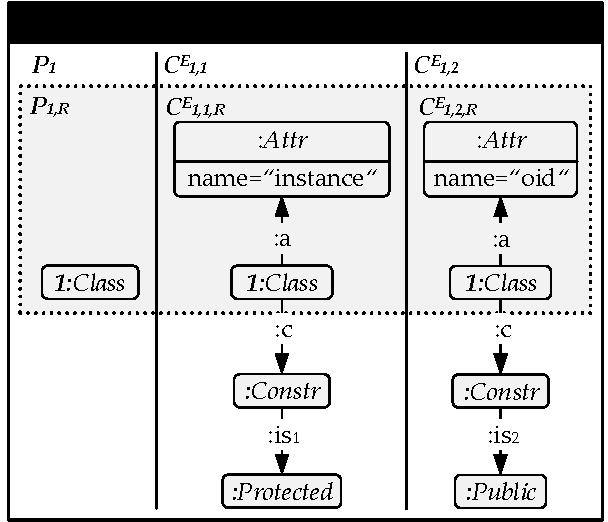
\includegraphics[width=.55\textwidth]{img/domain_res/res_ext.pdf}};
\fill (-1.25,3.15) node[inner sep=1pt] (B) {\textcolor{white}{$c_8=\vee_{i=(1,2)}(\exists(P_1 \to C^E_{1,i},\true))$}};
\end{tikzpicture}
\end{center}
\caption{Extended Domain Graph Constraint with Restriction}
\label{fig:sec-dc-general:res_ext}
\end{figure}

In \cref{sec-dom-compl-mt,thm:sec-dom-compl-mt:dom_compl_res_mt_II}, we instantiate the result from \cref{thm:sec-dc-general-res:dom_compl_res} to the domain completeness of model transformations under restrictions and show in \cref{sec-dom-compl-mt,fig:sec-dom-compl-mt:ex:dom_compl_1} that the transformation as defined by the $\TGG$ in \cref{fig:sec-dc-general:res_tg} is domain complete under restrictions if constraint $c_8$ from \cref{fig:sec-dc-general:res_ext} is added to the domain constraints in \cref{fig:sec-dc-general:res_c}.
This is necessary in order to obtain $C$-extension completeness for the example according to \cref{sec-dc-verification,def:C-extensionCompleteness}, i.e., to obtain extensions that can be created via the rules of the given $\TGG$.
Constraint $c_8$ is not contained in the initial set of domain constraints in \cref{fig:sec-dc-general:res_c}.
However, the constraint can be inferred from the initial set by performing $C$-extensions of the conclusion graphs of initial domain constraint $c_1$ via constraints $c_2$ and $c_3$ according to \cref{sec-dc-verification,def:C-extension}.
As in the example, the extension of domain constraints is useful for the verification of domain completeness under restrictions if the verification is based on the verification of domain completeness w.r.t. restricted domain constraints according to \cref{thm:sec-dc-general-res:dom_compl_res} and $C$-extension completeness cannot be successfully verified based on the initial set of restricted domain constraints but based on an extended set that additionally contains constraints that are inferred from initial constraints via elements outside the restriction, as it is the case for constraint $c_8$ where class constructors and their visibilities are taken into account for the inference but which are omitted in the restricted constraints.
Therefore, we propose to extend the initial set of domain constraints at first and then to use the refined set for verifying domain completeness under restrictions.
In \cref{def:sec-dc-general-res:ext_constr}, we define the step-wise extension of conditions and show in \cref{thm:sec-dc-general-res:ext_constr} that a graph satisfies the initial constraints if and only if it does also satisfy the extended constraints implying further that the language over the initial set of domain constraints equals to the language over the refined set.
Therefore, the refined set of constraints can be used instead of the initial set when verifying domain completeness.
Note that we restrict to extensions of plain conditions without multiple nestings.
However, we are confident that the approach can be extended to conditions with arbitrary nestings such that \cref{thm:sec-dc-general-res:ext_constr} holds, in future work.

\begin{definition}[$C$-Extensions of Conditions]
\label{def:sec-dc-general-res:ext_constr}
Let $\ac_P$ be a plain condition and $C$ be a set of conditions.
\emph{The extensions $Extensions(\ac_P,C)$ of $\ac_P$ via $C$}\index{graph condition!$C$-extensions} is inductively defined as follows based on the $C$-extensions of conclusion graphs according to \cref{sec-dc-verification,def:C-extension}:
$
  \begin{array}[t]{ll}
  Extensions(\ac_P,C) = \{\true\} & , \text{ for } \ac_P=\true, \\
  Extensions(\ac_P,C) = \{\vee_{i \in \{1,\ldots,n\}}(\exists(P \trans{e_i \circ a} E_i,\true)) \mid & , \text{ for } \ac_P=\exists(a\colon P \to C',\true),\\
  E=\{E_1,\ldots,E_n\} \in Extensions(C',C)\} \text{ where } e_i\colon C' \to E_i & \\
  \text{is the induced morphism according to \cref{sec-dc-verification,def:C-extension}} & \\
  Extensions(\ac_P,C) = \{\vee_{i \in I}(e_{P,i}) \mid e_{P,i} \in Extensions(\ac_{P,i},C)\} & , \text{ for } \ac_P=\vee_{i \in I}(\ac_{P,i}),\\
  Extensions(\ac_P,C) = \{\wedge_{i \in I}(e_{P,i}) \mid e_{P,i} \in Extensions(\ac_{P,i},C)\} & , \text{ for } \ac_P=\wedge_{i \in I}(\ac_{P,i}), and \\
  Extensions(\ac_P,C) = \{\neg e_P \mid e_P \in Extensions(\ac'_P,C)\} & , \text{ for } \ac_P=\neg\ac'_P.
  \end{array}
$
\envEndMarker
\end{definition}

\begin{example}[$C$-Extensions of Conditions]
The condition in \cref{fig:sec-dc-general:res_ext} is an extension of condition $c_1$ in \cref{fig:sec-dc-general:res_c} via conditions $c_2$ and $c_3$.
\envEndMarker
\end{example}

Note that in \cref{thm:sec-dc-general-res:ext_constr}, conditions are extended via conditions that are designated for general satisfaction only.
If we allow the extension of conditions via conditions that are designated for initial satisfaction, then \cref{thm:sec-dc-general-res:ext_constr} may not hold. 
For example, consider two constraints ``Each node \code{:A} is connected to two \code{:B} nodes'' and ``There exists a \code{:B} node connected to a \code{:C} node''.
The extension of the first constraint via the second constraint may lead to a constraint ``Each node \code{:A} is connected to two \code{:B} nodes and furthermore, each of the two \code{:B} nodes is connected to a \code{:C} node''.
Therefore, the existential characteristic of the \code{:B} node in the second constraint switches to a universal characteristic in the extended constraint.
Thus, a graph which satisfies the first initial constraint may not satisfy the extended constraint.

\begin{theorem}[Equivalence of Languages over Constraints \& Extended Constraints]
\label{thm:sec-dc-general-res:ext_constr}
In an $\M$-adhesive category with effective pushouts, let $C_I \cup C_G$ be a set of constraints where constraints $C_I$ are designated for initial satisfaction and constraints $C_G$ are designated for general satisfaction.
Furthermore, let $C'_I$ ($C'_G$) be a set of extensions of conditions $C_I$ ($C_G$) via $C_G$.
Then, it holds that $G \in \Lang_I(C_I) \cap \Lang(C_G)$ if and only if $G \in \Lang_I(C_I \cup C'_I) \cap \Lang(C_G \cup C'_G)$.
Therefore, $\Lang_I(C_I) \cap \Lang(C_G)=\Lang_I(C_I \cup C'_I) \cap \Lang(C_G \cup C'_G)$.
\envEndMarker
\end{theorem}

\begin{proof}
The proof is presented in \cref{sec-proofs:thm:sec-dc-general-res:ext_constr}.
\end{proof}
